\documentclass[journal]{IEEEtran}
\usepackage[T1]{fontenc}
\usepackage[utf8]{inputenc}
\usepackage{amsmath,amssymb}
\usepackage{graphicx}
\usepackage{booktabs}
\usepackage{array}
\usepackage{hyperref}
\usepackage{cite}
\usepackage{caption}
\usepackage{microtype}
\usepackage{xr}
\externaldocument[M-]{main_conference}
\emergencystretch=1em
\hypersetup{colorlinks=true, linkcolor=black, citecolor=black, urlcolor=black}

% S-numbering for floats and sections
\renewcommand{\thetable}{S\arabic{table}}
\renewcommand{\thefigure}{S\arabic{figure}}
\renewcommand{\thesection}{S\Roman{section}}

\begin{document}

\title{Supplementary Material for\\ ``Towards Trustworthy IoT Network Security:
Interpretable Open-Set Intrusion Detection''}
\author{Ngari~Crisphine~Macharia and~Ning~Weng}
\maketitle

\noindent This supplement provides the complete concept and rule definitions, the CTU-IoT-23
feature derivation, the threshold-gradient derivation, expanded ablations, per-class and
per-family results, and additional robustness analyses. The main article presents the
methods, principal evidence, and limitations supporting the central conclusions. Table,
figure, and section numbers here are prefixed ``S''; references to the main article use its
numbering.

\noindent\textbf{Feature set.} Following the known-class feature-selection control
(Section~\ref{sec:features}), all CTU-IoT-23 results in the main article and in the
finding-bearing supplementary tables (this control, the $\alpha$-gate sweep and head-agreement,
the per-family open-set breakdown, the concept-accuracy and leakage probe,
the temporal split and the $(\lambda,\gamma)$ grid) use the leak-free
known-class-only feature selection; the paired comparison with the originally submitted feature list
is the AUROC$^\S$ column of main Table~\ref{M-tab:main}. Every split is
drawn deterministically by the released scripts, and the released code includes a script that
prints every table value from the released results.

\section{The \texorpdfstring{$\alpha$}{alpha}-Gate and Interpretability Trade-Off}
\label{sec:alpha}

We sweep $\lambda_\alpha$ over six values, five seeds each
(Table~\ref{tab:alpha}). The regulariser raises the learned gate \emph{monotonically}.
On CTU-IoT-23, $\alpha$ rises from $0.38$ ($\lambda_\alpha{=}0$) to $0.89$
($\lambda_\alpha{=}1.0$); on CIC-IoT-2023, from $0.32$ to $0.95$. F1 does not move:
the known-class \emph{validation} F1 (the model-selection split reported in this sweep)
stays near $0.933$ on CTU and $0.818$--$0.819$ on CIC; the corresponding
held-out \emph{test} F1 is $0.933$ on CTU (Table~\ref{M-tab:main}). OOD AUROC is flat on CTU
(within $0.016$ across the sweep) and rises on CIC, from $0.647$ at
$\lambda_\alpha{=}0$ to $0.658$--$0.673$ for every $\lambda_\alpha{\ge}0.05$, a
gain of $0.01$--$0.03$ (up to about one seed std) that accompanies the increase in $\alpha$; as the
next paragraph shows, it is not evidence that the decision moved onto the rules.

\textbf{Does raising $\alpha$ actually move the decision onto the rules? No.} A larger
gate weight need not mean more rule reliance, because the two heads can emit logits of
different magnitudes and the learned weights can compensate. Testing reliance directly by
branch agreement (Table~\ref{tab:headagree}), the deployed known-class prediction (before
rejection) stays with the
\emph{neural-only} head at every $\lambda_\alpha$, and its agreement with the
\emph{rule-only} head rises only mildly as $\alpha$ increases (CTU $32\%$ to $51\%$),
staying well below neural agreement.
So $\lambda_\alpha$ tunes the gate scalar but not decision-level reliance on the rules;
we describe $\alpha$ as the learned rule-head weight in the logit blend, not as a measure
of how interpretable the decision is. (This is also a global scalar gate, so it cannot route
individual hard flows to the neural branch.) Each point was trained from scratch.

\begin{table}[t]
\centering\small
\caption{Branch agreement across the $\lambda_\alpha$ sweep (NeSy-NIDS, mean over five
seeds): learned $\alpha$ and the fraction of flows on which the deployed known-class prediction
(before rejection) equals the neural-only (dep$=$neural) or rule-only (dep$=$rule) prediction. The
open-set rejection score is computed on the hard rule vector, so these figures do not measure the
rules' influence on rejection.}
\label{tab:headagree}
\setlength{\tabcolsep}{4pt}
\resizebox{\columnwidth}{!}{%
\begin{tabular}{lcccccc}
\toprule
$\lambda_\alpha$ & 0 & 0.05 & 0.1 & 0.2 & 0.5 & 1.0 \\
\midrule
CTU $\alpha$              & 0.38 & 0.58 & 0.69 & 0.81 & 0.86 & 0.89 \\
CTU dep$=$neural          & 1.00 & 1.00 & 1.00 & 1.00 & 1.00 & 1.00 \\
CTU dep$=$rule            & 0.32 & 0.36 & 0.38 & 0.48 & 0.51 & 0.48 \\
CIC $\alpha$              & 0.32 & 0.81 & 0.86 & 0.90 & 0.93 & 0.95 \\
CIC dep$=$neural          & 0.99 & 0.98 & 0.97 & 0.98 & 0.98 & 0.97 \\
CIC dep$=$rule            & 0.45 & 0.52 & 0.53 & 0.53 & 0.52 & 0.55 \\
\bottomrule
\end{tabular}}
\end{table}

\begin{table}[t]
\centering\small
\setlength{\tabcolsep}{4pt}
\caption{$\alpha$-gate sweep (NeSy-NIDS, mean over five seeds): learned $\alpha$ and OOD
AUROC per $\lambda_\alpha$.}
\label{tab:alpha}
\begin{tabular}{lcccccc}
\toprule
$\lambda_\alpha$ & 0 & 0.05 & 0.1 & 0.2 & 0.5 & 1.0 \\
\midrule
CTU $\alpha$      & 0.38 & 0.58 & 0.69 & 0.81 & 0.86 & 0.89 \\
CTU AUROC         & 0.904 & 0.900 & 0.909 & 0.900 & 0.899 & 0.893 \\
CIC $\alpha$      & 0.32 & 0.81 & 0.86 & 0.90 & 0.93 & 0.95 \\
CIC AUROC         & 0.647 & 0.658 & 0.672 & 0.659 & 0.660 & 0.673 \\
\bottomrule
\end{tabular}
\end{table}

\begin{figure}[t]
  \centering
  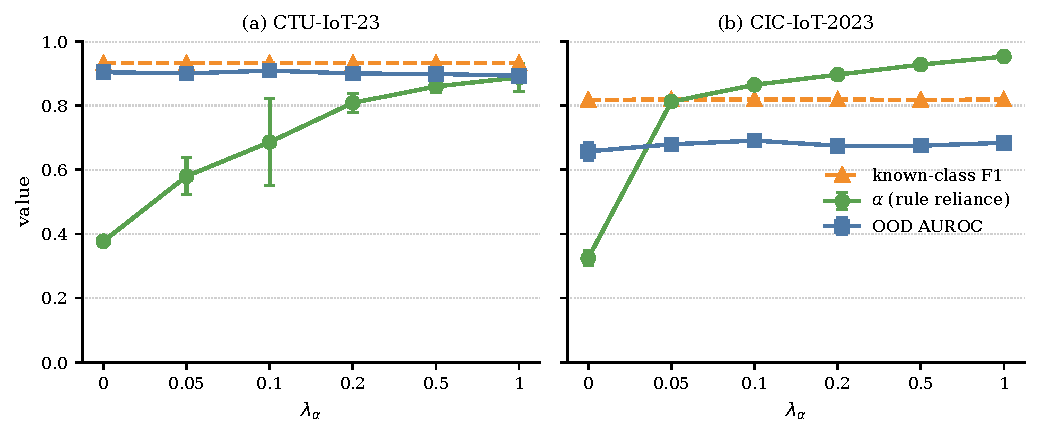
\includegraphics[width=\linewidth]{figures/alpha_sweep.pdf}
  \caption{$\alpha$-gate sweep (NeSy-NIDS, mean over five seeds; error bars
    $\pm$1 std). Raising $\lambda_\alpha$ drives the learned gate $\alpha$
    (the rule \emph{weight} in the logit blend, green) monotonically upward while
    known-class F1 (orange, dashed) stays flat and OOD AUROC (blue) is flat on
    CTU-IoT-23 but rises modestly on CIC-IoT-2023.}
  \label{fig:alpha_sweep}
\end{figure}

\section{Concept Leakage and the \texorpdfstring{$\gamma$}{gamma} Ablation}
\label{sec:leakage}

Table~\ref{tab:cbm_concepts} reports mean concept prediction accuracy for
each CBM variant over five seeds. This quantity is the \emph{concept accuracy} of the main text: agreement between the bottleneck's predicted concept and
the declared threshold label, i.e.\ how faithfully the model reproduces the
declared predicate, not whether the predicate is semantically ``correct''. JointCBM without concept regularisation
($\gamma{=}0$) reaches 87.4\% on CTU and 96.3\% on CIC. On CTU, accuracy rises
to 94.2\% at $\gamma{=}1.0$ (not monotonically: 89.1\% at $\gamma{=}0.1$, 88.9\% at $0.5$); at $\gamma{=}0$ the weakest concept
is \texttt{is\_persistent} at 81\% (it rises to 91\% by $\gamma{=}1.0$). On CIC it rises from 96.3\% to 97.2\%, with
every concept above 90\%. SequentialCBM reaches near-perfect concept accuracy
(99.9\% / 99.5\%) because its concept head is trained on the concept labels
alone and frozen before the classifier is trained. HybridCBM is similar
(99.6\% / 99.2\%): its skip connection lets the classifier bypass the
bottleneck, so the concept head is under less classification pressure and can
fit the concept labels more closely. Higher concept accuracy means closer agreement
with the threshold labels; as the OOD results show, it does not by itself buy
better detection.

\begin{table}[!t]
\renewcommand{\arraystretch}{1.0}
\caption{Mean concept prediction accuracy (\%) on the known-class test split
per CBM variant (mean over five seeds; $\lambda$ sensitivity in
Table~\ref{tab:lambdagamma}).}
\label{tab:cbm_concepts}
\centering
\small
\begin{tabular}{lcc}
\toprule
\textbf{Model} & \textbf{CTU-IoT-23} & \textbf{CIC-IoT-2023} \\
\midrule
JointCBM ($\gamma{=}0$)   & 87.4 & 96.3 \\
JointCBM ($\gamma{=}0.1$) & 89.1 & 96.5 \\
JointCBM ($\gamma{=}0.5$) & 88.9 & 96.8 \\
JointCBM ($\gamma{=}1.0$) & 94.2 & 97.2 \\
SequentialCBM             & 99.9 & 99.5 \\
HybridCBM                 & 99.6 & 99.2 \\
\bottomrule
\end{tabular}
\end{table}

Higher agreement with the labels does not by itself show that the bottleneck is free of
\emph{concept leakage}. We therefore train a linear classifier on the
training split to predict the class from (i) the soft predicted concepts
$\hat{\mathbf{c}}\in[0,1]^K$ and (ii) the same predictions thresholded at $0.5$, and report
the test-accuracy difference. This difference measures the additional predictive utility
of the continuous values for these probes. It is small on CTU-IoT-23 for $\gamma{\le}0.5$
(five-seed means $0.001$--$0.013$) but reaches $0.084{\pm}.088$ at $\gamma{=}1.0$, where two of five
seeds gain $0.17$--$0.21$; on CIC-IoT-2023 it is $0.04$--$0.06$ and grows rather than shrinks with
$\gamma$ ($\gamma{=}0$: $0.041{\pm}.008$; $\gamma{=}1.0$: $0.058{\pm}.008$).

A small difference does not establish semantic fidelity. Both probes use \emph{predicted}
concepts, and the thresholded predictions are not the declared predicates: where they
disagree with the declared labels, the pattern of disagreement can itself carry class
information. The predicate-replacement test of Section~\ref{sec:concept_intervention}
therefore uses the declared predicates directly.

\section{Temporal (Timestamp-Ordered) Split on CTU-IoT-23}
\label{sec:temporal}

The temporal split takes the main split's per-class sample, orders each known class by capture
timestamp (compared only within a class) and assigns its earliest 70\% to training, the next 15\% to
validation and the latest 15\% to test (five seeds; unknown families unchanged). Sessions or
captures may straddle the boundary, so we claim temporal ordering, not capture-, session- or
device-disjointness (Section~\ref{sec:device} holds out source addresses). The CTU \emph{DDoS} label
is temporally bimodal: a high-rate flood capture (September 2018, median Rate
${\approx}9.3{\times}10^{5}$\,pps) and near-zero-rate captures (December 2018 onward, median Rate
${<}1$), so the split trains on one regime and tests on the other, and every model scores F1 $0.00$
on DDoS on every seed; with the main 31-feature list only two JointCBM $\gamma{=}0.5$ seeds keep DDoS
(F1 $0.65$), so the cause is the label, not feature selection. Four-class F1 falls from $0.933$ to
$0.646$--$0.648$ for every model but SequentialCBM (C\&C-HeartBeat also falls, from $0.998$ to about
$0.79$), a temporal-generalisation cost rather than an interpretability one. On the three coherent
families the JointCBM variants, HybridCBM and NeSy-NIDS match the MLP (Coh-3 $0.862$--$0.863$) while
redistributing errors (e.g.\ $\gamma{=}0$: Benign $0.841$ vs.\ $0.958$, Okiru $0.961$ vs.\ $0.844$);
SequentialCBM loses Benign (F1$_4$ $0.330$, Coh-3 $0.441$). NeSy-NIDS gives the highest temporal-split
AUROC ($0.888{\pm}0.025$; $0.901{\pm}0.030$ with the $\alpha$ penalty).

\section{Source-IP Holdout}
\label{sec:device}

Flows are grouped by source IP address. Our merged flow tables keep the source IP but not the
capture name, and an address can recur across captures, so a held-out address is not shown to be
one physical device; the conclusions concern source addresses. CTU addresses 192.168.1.198 and
192.168.100.111 have at least $3{,}450$ flows in every known class; each in turn supplies the known
test set ($3{,}450$ per class), all other addresses supply the training and validation flows (for
.198 C\&C-HeartBeat has $14{,}699$ training flows instead of $16{,}100$), and the unknown test flows
are the main split's. Features are re-selected on each split's training rows (36 for .198, 33 for
.111), with the main 31-feature list (31f) as a control. The MLP, the CBM variants and NeSy-NIDS
(with the $\alpha$ penalty and the rule-only head) are trained with five seeds
(\texttt{06\_make\_kfs\_splits.py --split device}).

\begin{table}[h]
\centering\footnotesize
\caption{CTU source-IP holdout: known-class weighted F1 (five-seed mean) and OOD AUROC
(mean$\pm$std, five seeds) with the re-selected features, and AUROC with the main 31-feature list
(31f). With the 31-feature list, F1 is $0.417$ on address .198 ($0.517$ for NeSy-NIDS ($\alpha$)) and
$0.149$--$0.227$ on address .111. Main split for reference: F1 $0.566$--$0.933$, AUROC $0.805$--$0.909$.}
\label{tab:device}
\setlength{\tabcolsep}{3pt}
\resizebox{\columnwidth}{!}{%
\begin{tabular}{@{}lcccccc@{}}
\toprule
 & \multicolumn{3}{c}{Address 192.168.1.198} & \multicolumn{3}{c}{Address 192.168.100.111} \\
\cmidrule(lr){2-4}\cmidrule(lr){5-7}
Model & F1 & AUROC & AUROC 31f & F1 & AUROC & AUROC 31f \\
\midrule
MLP baseline               & $0.417$ & $0.528{\pm}.020$ & $0.529{\pm}.013$ & $0.228$ & $0.219{\pm}.045$ & $0.383{\pm}.015$ \\
JointCBM $\gamma{=}0$      & $0.417$ & $0.738{\pm}.113$ & $0.824{\pm}.081$ & $0.223$ & $0.211{\pm}.102$ & $0.111{\pm}.048$ \\
JointCBM $\gamma{=}0.1$    & $0.417$ & $0.809{\pm}.073$ & $0.770{\pm}.084$ & $0.214$ & $0.235{\pm}.085$ & $0.113{\pm}.043$ \\
JointCBM $\gamma{=}0.5$    & $0.417$ & $0.784{\pm}.050$ & $0.816{\pm}.083$ & $0.200$ & $0.256{\pm}.088$ & $0.114{\pm}.029$ \\
JointCBM $\gamma{=}1.0$    & $0.417$ & $0.819{\pm}.048$ & $0.789{\pm}.062$ & $0.196$ & $0.161{\pm}.015$ & $0.093{\pm}.028$ \\
SequentialCBM              & $0.417$ & $0.865{\pm}.001$ & $0.866{\pm}.002$ & $0.192$ & $0.170{\pm}.013$ & $0.202{\pm}.030$ \\
HybridCBM                  & $0.417$ & $0.821{\pm}.033$ & $0.822{\pm}.041$ & $0.152$ & $0.215{\pm}.038$ & $0.230{\pm}.042$ \\
NeSy-NIDS                  & $0.417$ & $0.843{\pm}.042$ & $0.846{\pm}.045$ & $0.161$ & $0.284{\pm}.043$ & $0.279{\pm}.044$ \\
NeSy-NIDS ($\alpha$)       & $0.417$ & $0.847{\pm}.045$ & $0.847{\pm}.045$ & $0.136$ & $0.278{\pm}.058$ & $0.280{\pm}.043$ \\
Rule-only                  & $0.416$ & $0.770{\pm}.032$ & $0.770{\pm}.032$ & $0.177$ & $0.193{\pm}.035$ & $0.193{\pm}.035$ \\
\bottomrule
\end{tabular}}
\end{table}

Known-class classification fails for every model. The held-out addresses' class traffic differs
from the other addresses': no Benign or DDoS test flow of .198, and no test flow of .111, has an
exact same-class duplicate in training (Section~\ref{sec:device2}), and .198's $3{,}450$ Benign test
flows are three distinct feature vectors. With the re-selected features every MLP, CBM and NeSy-NIDS
run scores F1 $0.00$ on .198's Benign (which the MLP labels Okiru) and on one more class, fixing
weighted F1 at $0.417$, and below $0.03$ on .111's DDoS and Okiru (which the MLP labels
C\&C-HeartBeat). AUROC then no longer isolates novel attack types: on .111 it is below $0.5$ in all
100 runs, because the held-out known flows look more novel than the unknown flows, over $99.9\%$ of
which come from addresses that also produce known traffic ($89\%$ for .198).

\subsection{A Third CTU Address and TON\_IoT}
\label{sec:device2}
Address 192.168.100.108 ($3{,}450$ flows per attack class, $3{,}051$ Benign, no unknown-family flows)
gives a third CTU fold. On TON\_IoT, \texttt{07\_make\_splits\_ton.py --holdout-attacker} takes
$7{,}500$ test flows per attack class from 192.168.1.30 or .31 and $7{,}500$ normal flows from .195 or
.190, training on all other addresses; NeSy-NIDS has no TON\_IoT rule bank.

\begin{table}[h]
\centering\footnotesize
\caption{CTU address .108 and the two TON\_IoT source-IP holdouts: known-class weighted F1 (five-seed
mean) and OOD AUROC against the main split's unknown pool (mean$\pm$std, five seeds). 31f: the
main 31-feature CTU list. TON\_IoT main split: F1 $0.704$--$0.898$, AUROC $0.552$--$0.654$.}
\label{tab:device2}
\setlength{\tabcolsep}{2.5pt}
\resizebox{\columnwidth}{!}{%
\begin{tabular}{@{}lccccccc@{}}
\toprule
 & \multicolumn{3}{c}{CTU address .108} & \multicolumn{2}{c}{TON\_IoT address .30} & \multicolumn{2}{c}{TON\_IoT address .31} \\
\cmidrule(lr){2-4}\cmidrule(lr){5-6}\cmidrule(lr){7-8}
Model & F1 & AUROC & AUROC 31f & F1 & AUROC & F1 & AUROC \\
\midrule
MLP baseline               & $0.544$ & $0.548{\pm}.003$ & $0.542{\pm}.008$ & $0.761$ & $0.552{\pm}.024$ & $0.886$ & $0.493{\pm}.033$ \\
JointCBM $\gamma{=}0$      & $0.541$ & $0.600{\pm}.030$ & $0.590{\pm}.122$ & $0.754$ & $0.635{\pm}.007$ & $0.885$ & $0.585{\pm}.012$ \\
JointCBM $\gamma{=}0.1$    & $0.539$ & $0.577{\pm}.056$ & $0.554{\pm}.071$ & $0.766$ & $0.659{\pm}.027$ & $0.853$ & $0.597{\pm}.026$ \\
JointCBM $\gamma{=}0.5$    & $0.547$ & $0.595{\pm}.068$ & $0.625{\pm}.037$ & $0.746$ & $0.664{\pm}.023$ & $0.858$ & $0.613{\pm}.033$ \\
JointCBM $\gamma{=}1.0$    & $0.546$ & $0.632{\pm}.059$ & $0.635{\pm}.050$ & $0.753$ & $0.660{\pm}.017$ & $0.888$ & $0.617{\pm}.011$ \\
SequentialCBM              & $0.343$ & $0.753{\pm}.049$ & $0.729{\pm}.031$ & $0.677$ & $0.596{\pm}.009$ & $0.731$ & $0.601{\pm}.016$ \\
HybridCBM                  & $0.544$ & $0.620{\pm}.049$ & $0.689{\pm}.077$ & $0.767$ & $0.610{\pm}.016$ & $0.892$ & $0.598{\pm}.020$ \\
NeSy-NIDS                  & $0.552$ & $0.907{\pm}.011$ & $0.899{\pm}.010$ & -- & -- & -- & -- \\
NeSy-NIDS ($\alpha$)       & $0.541$ & $0.906{\pm}.014$ & $0.898{\pm}.010$ & -- & -- & -- & -- \\
Rule-only                  & $0.475$ & $0.887{\pm}.011$ & $0.887{\pm}.011$ & -- & -- & -- & -- \\
\bottomrule
\end{tabular}}
\end{table}

On TON\_IoT the largest losses are on normal and password (address .30, MLP: normal $0.68$ vs.\
$0.91$, password $0.59$ vs.\ $0.79$); address .31 matches the main split. The share of known test
flows with an exact same-class training duplicate (features rounded to four decimals) is $0.84$ on
the CTU and $0.88$ on the TON\_IoT main split, $0.42$, $0.00$ and $0.41$ on CTU addresses .198, .111
and .108, and $0.74$ and $0.77$ on TON\_IoT addresses .30 and .31.

\subsection{Open-Set Test with Unknown Flows from the Held-Out Address}
\texttt{cbm/run\_device\_openset.py} scores each held-out address's known test flows against that
address's own unknown-family flows (MLP, CBMs, NeSy-NIDS): .198's $3{,}516$ ($3{,}499$ C\&C) and
$2{,}000$ DoS flows each from TON\_IoT .30 and .31, sampled as in the main split (their $2$ and $510$
MITM flows are scored separately). The seen-address reference scores the main-split models against
the main split's C\&C ($10{,}000$ of $21{,}995$) or DoS ($2{,}000$) flows; .111 and .108 lack
unknown-family flows. TPR@5\%FPR (Table~\ref{tab:devopen}), as in main Table~\ref{M-tab:main},
thresholds at the 95th percentile of the held-out address's own known test scores, a diagnostic
test-ROC point; Table~\ref{tab:devtau} uses the deployable threshold $\tau$ (main
Section~\ref{M-sec:openset}) set on validation flows of the training addresses.

\begin{table}[h]
\centering\footnotesize
\caption{OOD AUROC / diagnostic TPR@5\%FPR (five-seed mean) with known and unknown test flows from
the same source address. ``Seen'': main-split models against the same family's flows from
addresses seen in training. TON\_IoT columns use DoS flows only.}
\label{tab:devopen}
\setlength{\tabcolsep}{2.5pt}
\resizebox{\columnwidth}{!}{%
\begin{tabular}{@{}lcccccc@{}}
\toprule
 & \multicolumn{3}{c}{CTU, C\&C} & \multicolumn{3}{c}{TON\_IoT, DoS} \\
\cmidrule(lr){2-4}\cmidrule(lr){5-7}
Model & Seen & Address .198 & Address .198, 31f & Seen & Address .30 & Address .31 \\
\midrule
MLP baseline               & $0.853$ / $0.337$ & $0.396$ / $0.007$ & $0.396$ / $0.007$ & $0.444$ / $0.009$ & $0.411$ / $0.004$ & $0.818$ / $0.016$ \\
JointCBM $\gamma{=}0$      & $0.829$ / $0.339$ & $0.609$ / $0.052$ & $0.713$ / $0.162$ & $0.754$ / $0.016$ & $0.691$ / $0.007$ & $0.749$ / $0.016$ \\
JointCBM $\gamma{=}0.1$    & $0.832$ / $0.331$ & $0.663$ / $0.071$ & $0.688$ / $0.066$ & $0.735$ / $0.011$ & $0.705$ / $0.003$ & $0.757$ / $0.024$ \\
JointCBM $\gamma{=}0.5$    & $0.843$ / $0.439$ & $0.637$ / $0.020$ & $0.712$ / $0.100$ & $0.725$ / $0.014$ & $0.750$ / $0.002$ & $0.792$ / $0.026$ \\
JointCBM $\gamma{=}1.0$    & $0.854$ / $0.507$ & $0.690$ / $0.073$ & $0.665$ / $0.030$ & $0.735$ / $0.011$ & $0.703$ / $0.003$ & $0.772$ / $0.001$ \\
SequentialCBM              & $0.878$ / $0.497$ & $0.635$ / $0.039$ & $0.638$ / $0.041$ & $0.719$ / $0.022$ & $0.693$ / $0.000$ & $0.691$ / $0.002$ \\
HybridCBM                  & $0.876$ / $0.554$ & $0.636$ / $0.033$ & $0.637$ / $0.032$ & $0.722$ / $0.021$ & $0.690$ / $0.001$ & $0.645$ / $0.011$ \\
NeSy-NIDS                  & $0.865$ / $0.260$ & $0.651$ / $0.060$ & $0.651$ / $0.060$ & -- & -- & -- \\
NeSy-NIDS ($\alpha$)       & $0.872$ / $0.247$ & $0.651$ / $0.066$ & $0.650$ / $0.057$ & -- & -- & -- \\
Rule-only                  & $0.820$ / $0.183$ & $0.639$ / $0.031$ & $0.639$ / $0.031$ & -- & -- & -- \\
\bottomrule
\end{tabular}}
\end{table}

\begin{table}[h]
\centering\footnotesize
\caption{Deployable threshold $\tau$ (95th percentile of known validation scores): share of known
test flows rejected / recall of unknown flows (five-seed mean). The target rejection rate is 5\%.}
\label{tab:devtau}
\setlength{\tabcolsep}{2.5pt}
\resizebox{\columnwidth}{!}{%
\begin{tabular}{@{}lcccccc@{}}
\toprule
 & \multicolumn{3}{c}{CTU, C\&C} & \multicolumn{3}{c}{TON\_IoT, DoS} \\
\cmidrule(lr){2-4}\cmidrule(lr){5-7}
Model & Seen & Address .198 & Address .198, 31f & Seen & Address .30 & Address .31 \\
\midrule
MLP baseline               & $0.049$ / $0.337$ & $0.501$ / $0.049$ & $0.501$ / $0.049$ & $0.050$ / $0.009$ & $0.070$ / $0.004$ & $0.131$ / $0.070$ \\
JointCBM $\gamma{=}0$      & $0.048$ / $0.276$ & $0.250$ / $0.028$ & $0.051$ / $0.038$ & $0.052$ / $0.016$ & $0.062$ / $0.008$ & $0.060$ / $0.016$ \\
JointCBM $\gamma{=}0.1$    & $0.051$ / $0.335$ & $0.151$ / $0.027$ & $0.201$ / $0.033$ & $0.051$ / $0.016$ & $0.057$ / $0.003$ & $0.081$ / $0.037$ \\
JointCBM $\gamma{=}0.5$    & $0.052$ / $0.439$ & $0.200$ / $0.035$ & $0.151$ / $0.037$ & $0.051$ / $0.014$ & $0.060$ / $0.005$ & $0.058$ / $0.047$ \\
JointCBM $\gamma{=}1.0$    & $0.053$ / $0.513$ & $0.126$ / $0.131$ & $0.200$ / $0.033$ & $0.051$ / $0.017$ & $0.070$ / $0.006$ & $0.077$ / $0.003$ \\
SequentialCBM              & $0.055$ / $0.549$ & $0.000$ / $0.031$ & $0.000$ / $0.032$ & $0.051$ / $0.021$ & $0.099$ / $0.003$ & $0.062$ / $0.002$ \\
HybridCBM                  & $0.050$ / $0.552$ & $0.050$ / $0.026$ & $0.100$ / $0.027$ & $0.051$ / $0.021$ & $0.088$ / $0.004$ & $0.037$ / $0.002$ \\
NeSy-NIDS                  & $0.047$ / $0.286$ & $0.030$ / $0.042$ & $0.022$ / $0.041$ & -- & -- & -- \\
NeSy-NIDS ($\alpha$)       & $0.047$ / $0.268$ & $0.016$ / $0.040$ & $0.023$ / $0.040$ & -- & -- & -- \\
Rule-only                  & $0.039$ / $0.183$ & $0.177$ / $0.045$ & $0.177$ / $0.045$ & -- & -- & -- \\
\bottomrule
\end{tabular}}
\end{table}

On CTU the held-out address lowers C\&C AUROC from $0.82$--$0.88$ to $0.40$--$0.71$ and diagnostic
TPR from $0.18$--$0.55$ to at most $0.162$; on TON\_IoT address .30 the change is small (AUROC
$0.41$--$0.75$ vs.\ $0.44$--$0.75$), and TPR is low on seen addresses too ($\le0.022$). The deployable
threshold keeps known rejection near target on seen addresses ($3.9$--$5.5\%$) but not on held-out
ones ($0$--$50\%$ on .198, $3.7$--$13.1\%$ on TON\_IoT), with unknown recall at most $13.1\%$ (.198) and
$7.0\%$ (TON\_IoT). The model ordering is not stable across addresses (the concept models are above
the MLP on .198 and .30, below it on .31). On the $510$ MITM flows of .31, AUROC is $0.63$--$0.85$
and diagnostic TPR at most $0.139$.

\section{Confidence Intervals}
\label{sec:ci}
\texttt{cbm/run\_bootstrap\_ci.py} recomputes the per-flow OOD scores of every model compared from its saved
checkpoints (checked against the stored AUROC) and draws 2{,}000 hierarchical bootstrap replicates:
the five seeds are resampled with replacement for each model independently, and the $5{,}000$ known
and $5{,}000$ unknown evaluation flows are resampled with replacement and shared by the two models
of a comparison, since every model is scored on the same flows. The interval is the 2.5--97.5
percentile of the difference of the two seed-mean AUROCs. The intervals cover the variation from
training seeds and from the sampled evaluation flows under the chosen splits; they do not measure
uncertainty across new captures, source addresses or independently drawn splits.

\begin{table}[h]
\centering\footnotesize
\caption{Differences in mean OOD AUROC with 95\% bootstrap confidence intervals.}
\label{tab:ci}
\setlength{\tabcolsep}{3pt}
\resizebox{\columnwidth}{!}{%
\begin{tabular}{@{}llcc@{}}
\toprule
Data & Comparison & Difference & 95\% CI \\
\midrule
CTU & NeSy-NIDS $-$ MLP & $+0.030$ & $[+0.016, +0.043]$ \\
CTU & NeSy-NIDS ($\alpha$) $-$ MLP & $+0.035$ & $[+0.020, +0.047]$ \\
CTU & SequentialCBM $-$ MLP & $-0.002$ & $[-0.027, +0.018]$ \\
CTU & JointCBM $\gamma{=}1.0$ $-$ JointCBM $\gamma{=}0$ & $+0.011$ & $[-0.052, +0.065]$ \\
CTU & JointCBM $\gamma{=}0$ $-$ 8-unit bottleneck & $+0.263$ & $[+0.102, +0.380]$ \\
CIC & MLP $-$ JointCBM $\gamma{=}0$ & $+0.090$ & $[+0.073, +0.108]$ \\
CIC & JointCBM $\gamma{=}1.0$ $-$ JointCBM $\gamma{=}0$ & $-0.018$ & $[-0.037, +0.002]$ \\
CIC & 8-unit bottleneck $-$ JointCBM $\gamma{=}0$ & $+0.003$ & $[-0.024, +0.027]$ \\
CIC & NeSy-NIDS, energy score $-$ NeSy-NIDS, Mahalanobis & $+0.073$ & $[+0.035, +0.112]$ \\
TON & JointCBM $\gamma{=}0$ $-$ MLP & $+0.098$ & $[+0.051, +0.145]$ \\
TON & JointCBM $\gamma{=}0$ $-$ 8-unit bottleneck & $+0.106$ & $[+0.004, +0.214]$ \\
\bottomrule
\end{tabular}}
\end{table}

Every difference the main text describes as a gap excludes zero. An interval that includes zero
shows that this analysis does not resolve the difference, not that the two models are equivalent;
the main text describes those comparisons as similar observed AUROC or as no consistent
improvement. The TON\_IoT difference between JointCBM and
the 8-unit bottleneck barely excludes zero, because the bottleneck varies widely across seeds.

\section{Rule Selectivity and Threshold Drift}
\label{sec:selectivity}

All values in this section are mean binarised activations (Eq.~\ref{M-eq:binarise}) per
known class on the known-class validation split for the seed-0 model, the same data as
Fig.~\ref{M-fig:ruleactiv}. On CTU-IoT-23, several rules fire selectively but not deterministically
(\texttt{cc\_heartbeat\_beaconing} at $0.78$ and \texttt{incomplete\_handshake} at
$0.87$ on C\&C-HeartBeat, \texttt{asymmetric\_flood} at $0.81$ on DDoS and $0.13$ on Benign,
\texttt{ddos\_high\_rate} at $0.70$ on DDoS and $0.21$ on Okiru), leaving within-class
variance for Mahalanobis to work with; others fire across several classes
(\texttt{okiru\_low\_rate}: $0.79$ on Okiru but $0.87$ on Benign and $0.61$ on C\&C-HeartBeat). On CIC-IoT-2023 firing is
near-deterministic (\texttt{syn\_flood\_ddos} at $1.00$ on DDoS-SYN,
\texttt{benign\_low\_rate} at $0.97$ on Benign but also $0.91$ on Mirai), within-class variance is close to
zero, and Mahalanobis has little to separate on (AUROC $0.647$). These two activation
regimes coincide with the observed CTU-versus-CIC difference in Mahalanobis AUROC, but,
as the main paper establishes, known-class activation geometry does not by itself govern
detectability, so we report the pattern as descriptive, not causal
(Fig.~\ref{M-fig:ruleactiv}).
The learned thresholds move away from their expert initial values (seed~0): on
CTU-IoT-23 the \texttt{cc\_heartbeat\_beaconing} bounds move by up to $-0.50$, and on
CIC-IoT-2023 by up to $-0.88$ on \texttt{syn\_flood\_ddos}; across the five
seeds the per-condition drift vectors are correlated on CIC-IoT-2023 (mean pairwise $r{=}0.73$) but
not on CTU-IoT-23 ($r{=}0.05$; script \texttt{nesy/run\_fidelity.py}), so we read the CIC refinement as systematic
and the CTU pattern as indicative only (main Fig.~\ref{M-fig:threshdrift}).

\section{Configuration Sensitivity of the Geometry Correlations}
\label{sec:loco}

Main Table~\ref{M-tab:signflip} correlates each known-class statistic with OOD AUROC over
30 CBM models per dataset, which are five seeds of six configurations rather than 30
independent observations. Table~\ref{tab:loco} reports, on the same leak-free feature lists
as the main table (CTU: known-class-only selection, Section~\ref{sec:features}; CIC/TON:
fixed lists), two further aggregations applied identically to all three corpora: the
correlation over the six configuration means ($r_6$, $n{=}6$), and the range of the 30-model
correlation when each configuration in turn is excluded (leave-one-configuration-out, LOCO).
On CIC-IoT-2023 and TON\_IoT the seven statistics agree in direction, and the six separability
and variance statistics are strongly associated with AUROC at the configuration-mean level
($|r_6|\ge0.93$ on both); closed-set F1 is weaker ($r_6{=}0.63$ and $0.73$) and is the only
statistic whose sign changes under LOCO there (on CIC). CTU-IoT-23 is different. All seven
statistics take the opposite sign ($r_6$ from $-0.82$ to $+0.49$), and the LOCO ranges show why:
every CTU range reaches its bound closest to zero when SequentialCBM is excluded, where the
correlations fall to $|r|\le0.22$ and Fisher ratio, silhouette and closed-set F1 change sign.
SequentialCBM combines the least separable concept space and the lowest closed-set F1 with one
of the highest CTU AUROCs, so this single configuration sets the CTU direction. The
unknown/known ratio, which uses the unknown flows, is positive everywhere ($r_6$ $0.70$--$0.92$).
These are associations with Mahalanobis AUROC measured \emph{within} each corpus, and the strong
$r_6$ values rest on six points. Prediction on a held-out corpus and scorer selection are tested
separately (Sections~\ref{sec:lofo} and~\ref{sec:transfer}), and neither succeeds. The LOCO analysis thus
locates the CTU reversal in one configuration rather than in the corpus.

\begin{table}[t]
\centering\small
\caption{Configuration sensitivity of main Table~\ref{M-tab:signflip}, on the same leak-free
feature lists (CTU: known-class-only selection). $r_6$: Pearson $r$ over the six configuration
means. LOCO: range of the 30-model $r$ when one configuration is excluded; on CTU the bound
nearest zero is always the run without SequentialCBM. $^\ast$Sign changes when SequentialCBM is
excluded.}
\label{tab:loco}
\setlength{\tabcolsep}{3pt}
\resizebox{\columnwidth}{!}{%
\begin{tabular}{@{}lcccccc@{}}
\toprule
& \multicolumn{2}{c}{CTU-IoT-23} & \multicolumn{2}{c}{CIC-IoT-2023} & \multicolumn{2}{c}{TON\_IoT} \\
\cmidrule(lr){2-3}\cmidrule(lr){4-5}\cmidrule(lr){6-7}
Statistic & $r_6$ & LOCO & $r_6$ & LOCO & $r_6$ & LOCO \\
\midrule
Within-class variance & $+0.49$ & $[+0.01,+0.42]$ & $-0.96$ & $[-0.82,-0.66]$ & $-0.95$ & $[-0.54,-0.32]$ \\
Fisher ratio          & $-0.45$ & $[-0.32,+0.02]^\ast$ & $+0.96$ & $[+0.56,+0.76]$ & $+0.95$ & $[+0.36,+0.54]$ \\
Ridge-LDA             & $-0.50$ & $[-0.44,-0.08]$ & $+0.95$ & $[+0.31,+0.60]$ & $+0.98$ & $[+0.40,+0.57]$ \\
Silhouette            & $-0.46$ & $[-0.42,+0.01]^\ast$ & $+0.95$ & $[+0.74,+0.85]$ & $+0.94$ & $[+0.40,+0.58]$ \\
Nearest-centroid margin & $-0.47$ & $[-0.43,-0.02]$ & $+0.94$ & $[+0.50,+0.74]$ & $+0.94$ & $[+0.32,+0.52]$ \\
Concept entropy       & $-0.52$ & $[-0.47,-0.06]$ & $+0.96$ & $[+0.71,+0.83]$ & $+0.93$ & $[+0.25,+0.49]$ \\
Closed-set F1         & $-0.82$ & $[-0.42,+0.22]^\ast$ & $+0.63$ & $[-0.28,+0.76]^\ast$ & $+0.73$ & $[+0.03,+0.42]$ \\
\midrule
Unknown/known ratio   & $+0.78$ & $[+0.59,+0.74]$ & $+0.92$ & $[+0.43,+0.64]$ & $+0.70$ & $[+0.70,+0.76]$ \\
\bottomrule
\end{tabular}}
\end{table}

\section{CTU-IoT-23 Feature Derivation}
\label{sec:features}

CTU-IoT-23 is distributed as packet captures with labelled Zeek \texttt{conn.log} files. For
each capture we compute per-flow packet statistics with DPKT (field names follow the
CIC-IoT-2023 feature set) and join each labelled Zeek record to the DPKT flows with the same
source and destination IP, ports and protocol whose start time lies in $[t_{\mathrm{zeek}}{-}\mathrm{duration}{-}60\,\mathrm{s},\,
t_{\mathrm{zeek}}{+}60\,\mathrm{s}]$, keeping the one closest in start time
(\texttt{preprocess/merge\_iot23\_outer2.py}), so each Zeek record yields at most one row; in the
stored table only two pairs of rows share source address, timestamp, duration, byte counts, history and label. Zeek records without a DPKT match are
kept, with their DPKT features set to 0: 1{,}896{,}696 of the 110{,}879{,}826 retained flows ($1.7\%$), mostly
DDoS ($7.6\%$ of DDoS flows); no flow matched with protocol ICMP. In the main split they are
$2.2\%$ of the training and $2.0\%$ of the known test flows (mostly DDoS) and $0.4\%$ of the
unknown flows. Before sampling, a label filter excludes PartOfAHorizontalPortScan,
PartOfAHorizontalPortScan-Attack and C\&C-PartOfAHorizontalPortScan, so horizontal port scanning
is neither a known nor a held-out class. We used the full IoT-23 archive
(\texttt{iot\_23\_datasets\_full.tar.gz}), whose packet captures the DPKT features require, and keep
the labels of its Zeek label files. For capture CTU-IoT-Malware-Capture-33-1 these files label
$13{,}609{,}467$ flows Okiru, a count the provider's summary table lists under Okiru-Attack; our
flows from that capture's source address (192.168.1.197) include exactly $13{,}609{,}467$ Okiru and
no Okiru-Attack flows, and the label file for this capture currently served by the provider also
uses Okiru. These flows therefore belong to the known Okiru class, and our three Okiru-Attack flows
are those of capture 36-1; Table~\ref{tab:ctu_labels} lists the retained labels
(\texttt{checks/ctu\_label\_counts.py}).

\begin{table}[h]
\centering\footnotesize
\caption{Retained CTU-IoT-23 flows per label and those without a matching DPKT flow (DPKT
features set to 0).}
\label{tab:ctu_labels}
\begin{tabular}{@{}lrr@{}}
\toprule
Label & Retained & No DPKT match \\
\midrule
Okiru & 60{,}717{,}929 & 267{,}008 \\
Benign & 30{,}830{,}238 & 158{,}334 \\
DDoS & 19{,}265{,}778 & 1{,}471{,}222 \\
C\&C-HeartBeat & 33{,}537 & 6 \\
C\&C & 21{,}995 & 103 \\
Attack & 9{,}398 & 1 \\
C\&C-HeartBeat-Attack & 834 & 18 \\
C\&C-FileDownload & 53 & 4 \\
C\&C-Torii & 30 & 0 \\
FileDownload & 18 & 0 \\
C\&C-HeartBeat-FileDownload & 11 & 0 \\
Okiru-Attack & 3 & 0 \\
C\&C-Mirai & 2 & 0 \\
\bottomrule
\end{tabular}
\end{table}

 Four ratios are derived from Zeek fields: byte ratio
$\mathrm{orig\_bytes}/(\mathrm{resp\_bytes}{+}1)$, originator packet and byte rates
$\mathrm{orig\_pkts}/(\mathrm{duration}{+}1)$ and $\mathrm{orig\_ip\_bytes}/(\mathrm{duration}{+}1)$,
and direction $\mathrm{orig\_bytes}{-}\mathrm{resp\_bytes}$. The model uses 34 numeric features
(Zeek: duration, orig/resp bytes, packets and IP bytes; DPKT: Rate, Srate, IAT, Number,
Tot\_sum, Min, Max, AVG, Std, Variance, Magnitude, Radius, ack/syn/fin/rst counts,
fin/rst flag numbers, and HTTP, HTTPS, SSH, IRC, Telnet indicators; plus the four derived
ratios) and three Zeek categorical fields (conn\_state, history, service) integer-encoded, 37
in total. Missing values are set to $-1$; features are not rescaled.

\begin{sloppypar}\textbf{Feature-selection control.} The 34 numeric features were chosen before this study by a
class-weighted random forest (99\% of cumulative importance) trained on up to $10^6$ flows of every
labelled CTU family, including the nine later held out, so the submitted list is not blind to the
held-out labels (CIC-IoT-2023 and TON\_IoT use fixed lists). We therefore re-ran the same selection
on the known-class training rows only: the resulting list keeps 28 of the numeric features (it
drops HTTP, HTTPS, SSH, IRC, \texttt{resp\_pkts}, \texttt{fin\_count}, Radius, Std, Variance,
\texttt{resp\_ip\_bytes} and \texttt{rst\_flag\_number}, and adds TCP, Protocol\_Type, Time\_To\_Live
and the \texttt{cwr} and \texttt{syn} flag numbers), 31 features with the three categorical fields
(\texttt{ctuk}). The submitted list on the same rows (\texttt{ctuko}) isolates the selection source
from the sample. NeSy-NIDS keeps its expert rule features, so the two rule counters the known-only
forest drops are restored (\texttt{06\_make\_kfs\_splits.py}, \texttt{cbm/run\_kfs\_control.py},
\texttt{nesy/run\_kfs\_control.sh}). Main Table~\ref{M-tab:main} reports the outcome over five seeds
(F1; AUROC$^\S$ for \texttt{ctuko}). Known-class F1 is unchanged; per-class Mahalanobis remains the best
CTU scorer for every architecture (Table~\ref{tab:kfs_scorer}); $\gamma$ still has no monotone
effect. All OOD AUROC changes of $0.05$ or more are gains under known-class-only selection
(SequentialCBM $0.782{\pm}.042{\to}0.872{\pm}.026$, HybridCBM $0.772{\pm}.073{\to}0.822{\pm}.055$,
Post-hoc CBM $0.805{\to}0.871$); the MLP moves $-0.020$, NeSy-NIDS $+0.019$ ($0.885{\to}0.904$). The
submitted list therefore did not flatter the CTU detection results.\end{sloppypar}

\textbf{Per-split selection.} The same selection is re-run separately for each other CTU
experiment: on the alternative known set's training rows, the earliest 70\% of the temporal split
and each leave-one-family-out fold's reduced known set, so no held-out family or test-period flow
informs its features. The alternative split draws its own class-balanced sample, the temporal split
reorders the main split's sample by time, and the leave-one-family-out folds reuse the main split's
rows; for the alternative and temporal splits, the main 31-feature list on the same rows is a
control, and the accuracy, scorer and $\gamma$ conclusions hold under both.

\begin{table}[t]
\centering\footnotesize
\caption{Scorer comparison under the known-only feature selection (\texttt{ctuk}): OOD AUROC
(mean${\pm}$std, five seeds) for per-class Mahalanobis on the concept space, the logit-space
energy score, and their average after $z$-normalising each with known validation scores (combined). Per-class Mahalanobis is best for every
architecture, and the logit-energy score reaches at most $0.61$ (main
Table~\ref{M-tab:scorer_arch} gives the CIC comparison, where the ranking depends on architecture).}
\label{tab:kfs_scorer}
\setlength{\tabcolsep}{4pt}
\begin{tabular}{lccc}
\toprule
Architecture & Mahalanobis & Energy & Combined \\
\midrule
MLP                 & $\mathbf{0.879{\pm}.001}$ & $0.386{\pm}.073$ & $0.682{\pm}.046$ \\
JointCBM ($\gamma{=}0$)   & $\mathbf{0.830{\pm}.044}$ & $0.476{\pm}.111$ & $0.631{\pm}.068$ \\
JointCBM ($\gamma{=}0.1$) & $\mathbf{0.812{\pm}.034}$ & $0.494{\pm}.136$ & $0.624{\pm}.098$ \\
JointCBM ($\gamma{=}0.5$) & $\mathbf{0.851{\pm}.037}$ & $0.570{\pm}.138$ & $0.714{\pm}.106$ \\
JointCBM ($\gamma{=}1$)   & $\mathbf{0.842{\pm}.049}$ & $0.612{\pm}.124$ & $0.708{\pm}.100$ \\
SequentialCBM       & $\mathbf{0.875{\pm}.026}$ & $0.604{\pm}.085$ & $0.757{\pm}.018$ \\
HybridCBM           & $\mathbf{0.827{\pm}.055}$ & $0.365{\pm}.047$ & $0.610{\pm}.047$ \\
\bottomrule
\end{tabular}
\end{table}

\section{NeSy-NIDS Rule Bank and Initial Thresholds}
\label{sec:rulebank}

Table~\ref{tab:rulebank} gives the complete eight-rule bank for each dataset used by
NeSy-NIDS (Section~\ref{M-sec:nesy} of the main paper lists only representative rules). Each
rule is a conjunction of threshold conditions on named flow features; the thresholds shown
are the expert \emph{initial} values $\boldsymbol{\theta}^{(0)}$, which are then refined by
gradient descent through the $k$-annealed gates. The full feature
lists (per-dataset \texttt{feature\_cols}), the deterministic concept/rule threshold
values, and the train/val/test split indices are released with the code (see the
code-availability statement), so every representation in the paper is reproducible.

\begin{table}[t]
\centering\small
\caption{Complete NeSy-NIDS rule bank ($R{=}8$ per dataset): target class and the
conjunction of conditions at the expert \emph{initial} thresholds (refined during
training). CTU-IoT-23 in raw units; CIC-IoT-2023 in $z$-scored units.}
\label{tab:rulebank}
\setlength{\tabcolsep}{4pt}
\resizebox{\columnwidth}{!}{%
\begin{tabular}{@{}lll@{}}
\toprule
Rule & Target & Condition (initial threshold) \\
\midrule
\multicolumn{3}{@{}l}{\textbf{CTU-IoT-23} (raw units)} \\
ddos\_high\_rate         & DDoS         & Rate${>}1000$ \\
cc\_heartbeat\_beaconing & C\&C-HB      & $1.5{<}$IAT${<}5.0 \wedge 0.1{<}$Rate${<}5.0$ \\
benign\_single\_probe    & Benign       & orig\_pkts${<}2 \wedge$ Rate${<}100$ \\
okiru\_low\_rate         & Okiru        & Rate${<}500 \wedge$ duration${<}2.5$ \\
asymmetric\_flood        & DDoS         & resp\_pkts${<}1 \wedge$ orig\_pkts${>}1$ \\
persistent\_connection   & C\&C-HB      & duration${>}2.5$ \\
incomplete\_handshake    & C\&C-HB      & syn\_count${>}2 \wedge$ fin\_count${<}1$ \\
ddos\_short\_burst       & DDoS         & Rate${>}1000 \wedge$ duration${<}0.1$ \\
\midrule
\multicolumn{3}{@{}l}{\textbf{CIC-IoT-2023} ($z$-scored units)} \\
syn\_flood\_ddos         & DDoS-SYN     & rate${>}0.15 \wedge$ syn\_count${>}1.5$ \\
udp\_mirai\_flood        & Mirai        & tcp${<}{-}1.0 \wedge$ rate${>}0.0$ \\
recon\_port\_scan        & Recon        & rst\_count${>}1.5$ \\
vuln\_scan               & VulnScan     & fin\_count${>}1.0 \wedge$ rate${>}0.0$ \\
benign\_low\_rate        & Benign       & rate${<}0.0 \wedge$ syn\_count${<}0.0$ \\
large\_payload\_flood    & Benign       & avg${>}0.4 \wedge$ udp${>}0.0$ \\
high\_entropy\_scan      & Recon        & variance${>}0.5 \wedge$ rst\_count${>}0.5$ \\
short\_connection\_flood & DDoS-SYN     & iat${<}{-}0.003 \wedge$ rate${>}0.1$ \\
\bottomrule
\end{tabular}}
\end{table}

\section{Threshold Gradient}
\label{sec:gradient}

Training uses the soft activations of main Eq.~\ref{M-eq:rule_score} throughout, so every
threshold receives a gradient. For a greater-than condition $i\in\mathcal{I}_r^{>}$ of rule $r$,
\begin{equation}
  \frac{\partial \mathcal{L}}{\partial \theta_i} =
    \frac{\partial \mathcal{L}}{\partial a_r} \cdot
    \Bigl(-k(t)\,g_i^{>}(1{-}g_i^{>})\prod_{j \neq i} g_j\Bigr),
\end{equation}
where $g_i^{>}{=}\sigma(k(t)(x_i{-}\theta_i))$ and $g_j$ are the other gates of the rule; the
sign flips for less-than conditions. As $k(t)$ grows, $g_i^{>}(1{-}g_i^{>})$ vanishes for gates
far from their threshold, so late in training only borderline conditions keep moving. The
straight-through estimator is not used in training.

\section{Scorer Settings}
\label{sec:scorers}
Table~\ref{tab:scorers} lists how each OOD score is computed. Every setting was fixed in advance
(the ODIN and $k$NN values are the published defaults) and none was chosen using the held-out
families; scorers are fitted on training vectors, and the combined score is normalised with
known validation scores, so no test flow enters any scorer.

\begin{table}[h]
\centering\footnotesize
\caption{OOD scorer settings.}
\label{tab:scorers}
\setlength{\tabcolsep}{3pt}
\resizebox{\columnwidth}{!}{%
\begin{tabular}{@{}lp{0.72\columnwidth}@{}}
\toprule
Scorer & Computation \\
\midrule
Mahalanobis & Per-class means and a shared covariance of the within-class residuals ($+10^{-4}I$,
pseudo-inverse), fitted on $20{,}000$ training vectors; score $=$ distance to the nearest class mean \\
Hamming, Jaccard & Hard rule vectors; each class representative is the majority vote of its
training vectors (rule mean $>0.5$, so it is binary); score $=$ Hamming or Jaccard distance to the
nearest representative \\
Energy & $-\log\sum_c e^{l_c}$ on the logits, $T{=}1$ \\
Combined & Mahalanobis and energy scores each $z$-normalised with the mean and standard deviation
of the known validation scores (frozen before testing), then summed \\
MSP & $1-\max_c \mathrm{softmax}(l)_c$ \\
ODIN & MSP at temperature $T{=}1000$ after an input perturbation of $\epsilon{=}0.0014$ along the
sign of the gradient \\
$k$NN & Euclidean distance to the 50th nearest $L_2$-normalised training embedding ($20{,}000$
training vectors) \\
\bottomrule
\end{tabular}}
\end{table}

\section{Leave-Family-Out Scorer Selection}
\label{sec:lofo}

The measured associations between known-class statistics and OOD AUROC vary across
datasets (main Table~\ref{M-tab:signflip}); whether a scorer can be \emph{selected} in advance is a separate
question, which we test directly with a \emph{behavioural} proxy: hold out one known attack
family, retrain JointCBM
($\gamma{=}0$) on the reduced known set, and keep the scorer (per-class Mahalanobis vs
logit-space energy) that best detects the held-out family, then ask whether that choice
matches the scorer actually best on the true unknowns (Mahalanobis on CTU-IoT-23, energy
on CIC-IoT-2023). We repeat for every known attack family $\times$ five seeds
(main Table~\ref{M-tab:lofo}).

The proxy is only \emph{conditionally} reliable. On CTU-IoT-23 the family-majority vote
recovers Mahalanobis (two of three families, $9/15$ runs); the C\&C-HeartBeat and DDoS
held-out-family experiments favour it, and only Okiru misfires (Mahalanobis cannot detect held-out Okiru,
$0.22$). On CIC-IoT-2023 the family-majority vote selects Mahalanobis for all four families
($15/20$ runs, $5/20$ energy) and so never recovers energy: held-out known families
remain separable in activation space (Mahalanobis $0.70$--$0.86$), so the proxy selects
Mahalanobis, yet the true CIC unknowns overlap the known boundary and need energy. Held-out-known thus
over-approximates activation-space detectability exactly on the corpus where the scorer
must switch. In these experiments, therefore, this leave-family-out proxy did not
consistently identify the best scorer; selecting it reliably
would require observing the novel regime, which we do not demonstrate a priori. This is a
further instance of the paper's negative result, here for scorer \emph{selection} rather
than scorer performance. Driver: \texttt{cbm/run\_lofo.py}. A second rule that needs no
retraining, based on synthetic outliers, is evaluated in Section~\ref{sec:transfer}.

\section{Transfer and Selection Tests}
\label{sec:transfer}

\textbf{Transfer across corpora.} For each known-class statistic $s$ we fit
$\mathrm{AUROC}=a+b\,s$ by least squares on the 60 CBM concept-space models of two corpora and apply
it to the 30 models of the third (Table~\ref{tab:transfer}; \texttt{cbm/run\_geometry\_transfer.py}).
The prediction beats the training-corpora mean AUROC in $3$ of $21$ cases, ranks the held-out models
in the right direction in $7$ of $21$, and identifies the best configuration in $1$ of $21$. The
slope is dominated by between-corpus differences (the dataset means are non-monotone), so it often
has the wrong sign even for CIC-IoT-2023 and TON\_IoT, whose within-corpus directions agree.

\begin{table}[t]
\centering\footnotesize
\caption{Leave-one-corpus-out prediction of OOD AUROC from each known-class statistic (fitted on
the other two corpora, 60 models; evaluated on the 30 held-out models). Slope: fitted $b$; MAE:
mean absolute AUROC error on the held-out corpus; $\rho$: Spearman correlation of predicted and
true AUROC; Best: the predicted best configuration is the true best.}
\label{tab:transfer}
\setlength{\tabcolsep}{4pt}
\begin{tabular}{lcccc}
\toprule
Statistic & Slope & MAE & $\rho$ & Best \\
\midrule
\multicolumn{5}{@{}l}{\textbf{Held out: CTU} (training-mean MAE $0.167$)} \\
Within-class variance & $-1.774$ & $0.198$ & $-0.36$ & no \\
Fisher ratio & $+0.065$ & $0.169$ & $-0.34$ & no \\
Ridge-LDA & $+0.000$ & $0.180$ & $-0.38$ & no \\
Silhouette & $+0.336$ & $0.149$ & $-0.34$ & no \\
Nearest-centroid margin & $+0.201$ & $0.152$ & $-0.28$ & no \\
Concept entropy & $+0.006$ & $0.167$ & $-0.38$ & no \\
Closed-set F1 & $-0.022$ & $0.168$ & $+0.17$ & yes \\
\multicolumn{5}{@{}l}{\textbf{Held out: CIC} (training-mean MAE $0.045$)} \\
Within-class variance & $+0.616$ & $0.030$ & $-0.66$ & no \\
Fisher ratio & $+0.060$ & $0.075$ & $+0.60$ & no \\
Ridge-LDA & $+0.003$ & $0.671$ & $+0.41$ & no \\
Silhouette & $+0.263$ & $0.069$ & $+0.75$ & no \\
Nearest-centroid margin & $+0.247$ & $0.083$ & $+0.54$ & no \\
Concept entropy & $-0.415$ & $0.064$ & $-0.70$ & no \\
Closed-set F1 & $-0.006$ & $0.045$ & $-0.17$ & no \\
\multicolumn{5}{@{}l}{\textbf{Held out: TON} (training-mean MAE $0.123$)} \\
Within-class variance & $+2.001$ & $0.146$ & $-0.46$ & no \\
Fisher ratio & $-0.045$ & $0.145$ & $-0.51$ & no \\
Ridge-LDA & $-0.000$ & $0.153$ & $-0.58$ & no \\
Silhouette & $-0.092$ & $0.136$ & $-0.43$ & no \\
Nearest-centroid margin & $-0.113$ & $0.149$ & $-0.39$ & no \\
Concept entropy & $+0.113$ & $0.130$ & $+0.37$ & no \\
Closed-set F1 & $+0.128$ & $0.125$ & $+0.30$ & no \\
\bottomrule
\end{tabular}
\end{table}

\textbf{Scorer selection from synthetic outliers.} As a second known-traffic rule that needs no
retraining, we select Mahalanobis or energy by which better separates validation flows from
synthetic outliers: feature-wise permutations of validation flows (primary, fixed in advance) or
midpoints of random pairs (Table~\ref{tab:selection}; \texttt{cbm/run\_scorer\_selection.py}). Against
the scorer better on the true unknowns, the permutation rule is right for $25/35$ CTU, $26/35$ CIC
and $9/35$ TON\_IoT models ($60/105$), the midpoint rule for $27/35$, $21/35$ and $9/35$ ($57/105$);
always choosing Mahalanobis is right for $62/105$ and energy for $43/105$, and wrong permutation
choices cost $0.066$ AUROC on average. Both rules prefer Mahalanobis on TON\_IoT, where energy is
better for every architecture.

\begin{table}[t]
\centering\footnotesize
\caption{Scorer selection from synthetic outliers (five seeds). True: OOD AUROC on the held-out
unknown families; Perm.: AUROC separating validation flows from feature-permuted copies;
Correct: seeds on which the rule picks the scorer that is better on the true unknowns
(permutation / midpoint rule).}
\label{tab:selection}
\setlength{\tabcolsep}{3pt}
\resizebox{\columnwidth}{!}{%
\begin{tabular}{lcccccc}
\toprule
& \multicolumn{2}{c}{True} & \multicolumn{2}{c}{Perm.} & \multicolumn{2}{c}{Correct} \\
\cmidrule(lr){2-3}\cmidrule(lr){4-5}\cmidrule(lr){6-7}
Architecture & Mahal. & Energy & Mahal. & Energy & Perm. & Mid. \\
\midrule
\multicolumn{7}{@{}l}{\textbf{CTU-IoT-23}} \\
MLP & 0.879 & 0.386 & 0.984 & 0.766 & 5/5 & 4/5 \\
JointCBM ($\gamma{=}0$) & 0.830 & 0.476 & 0.802 & 0.703 & 4/5 & 4/5 \\
JointCBM ($\gamma{=}0.1$) & 0.812 & 0.494 & 0.795 & 0.747 & 3/5 & 4/5 \\
JointCBM ($\gamma{=}0.5$) & 0.851 & 0.570 & 0.823 & 0.747 & 4/5 & 5/5 \\
JointCBM ($\gamma{=}1.0$) & 0.842 & 0.612 & 0.853 & 0.786 & 5/5 & 5/5 \\
SequentialCBM & 0.875 & 0.604 & 0.644 & 0.585 & 4/5 & 4/5 \\
HybridCBM & 0.827 & 0.365 & 0.651 & 0.801 & 0/5 & 1/5 \\
\multicolumn{7}{@{}l}{\textbf{CIC-IoT-2023}} \\
MLP & 0.807 & 0.615 & 0.974 & 0.655 & 5/5 & 5/5 \\
JointCBM ($\gamma{=}0$) & 0.722 & 0.734 & 0.769 & 0.803 & 3/5 & 3/5 \\
JointCBM ($\gamma{=}0.1$) & 0.705 & 0.732 & 0.779 & 0.821 & 4/5 & 2/5 \\
JointCBM ($\gamma{=}0.5$) & 0.706 & 0.757 & 0.771 & 0.826 & 5/5 & 1/5 \\
JointCBM ($\gamma{=}1.0$) & 0.702 & 0.769 & 0.778 & 0.820 & 5/5 & 0/5 \\
SequentialCBM & 0.665 & 0.636 & 0.723 & 0.689 & 4/5 & 5/5 \\
HybridCBM & 0.670 & 0.629 & 0.678 & 0.732 & 0/5 & 5/5 \\
\multicolumn{7}{@{}l}{\textbf{TON\_IoT}} \\
MLP & 0.550 & 0.662 & 0.859 & 0.523 & 0/5 & 0/5 \\
JointCBM ($\gamma{=}0$) & 0.644 & 0.713 & 0.740 & 0.621 & 1/5 & 0/5 \\
JointCBM ($\gamma{=}0.1$) & 0.640 & 0.674 & 0.758 & 0.624 & 3/5 & 2/5 \\
JointCBM ($\gamma{=}0.5$) & 0.641 & 0.694 & 0.770 & 0.630 & 2/5 & 2/5 \\
JointCBM ($\gamma{=}1.0$) & 0.642 & 0.706 & 0.758 & 0.637 & 1/5 & 1/5 \\
SequentialCBM & 0.603 & 0.640 & 0.730 & 0.637 & 0/5 & 2/5 \\
HybridCBM & 0.615 & 0.641 & 0.747 & 0.548 & 2/5 & 2/5 \\
\bottomrule
\end{tabular}}
\end{table}

\section{Open-Set (C+1) and Per-Family Evaluation}
\label{sec:openset_supp}

\textbf{Protocol.} The deployed $(C{+}1)$-class detector rejects a flow as unknown if its
per-class Mahalanobis score (concept activations for the CBMs, hard rule activations for NeSy-NIDS,
the embedding for the MLP) exceeds $\tau$, the 95th percentile on known validation flows, and
otherwise takes the $\arg\max$ known-class logit. It is evaluated on $5{,}000$ known test flows and
up to $3{,}000$ flows per held-out family, all families merged into one unknown class (9 on CTU, 29
on CIC; main Table~\ref{M-tab:openset_agg}).

The known rejection rate is close to target ($4.2$--$5.8\%$; the coefficient of variation of $\tau$
across seeds is at most $0.11$). Open-set macro-F1 is $0.49$--$0.79$ on CTU-IoT-23 and $0.13$--$0.27$
on CIC-IoT-2023, largely a prevalence effect. For NeSy-NIDS on CIC-IoT-2023 (Table~\ref{tab:confusion},
seed 0) the pool has $5{,}000$ known and $84{,}514$ unknown flows, of which $15{,}646$ ($18.5\%$)
exceed $\tau$; the ${\sim}81\%$ not rejected are absorbed into known classes, and since unknowns
outnumber knowns ${\sim}17{:}1$ they collapse known-class precision (Benign $\approx0.07$, F1
$\approx0.13$), while the unknown class has the highest per-class F1 ($\approx0.31$). Reweighting the
same matrix to equal known and unknown totals, with all conditional rates unchanged, raises macro-F1
from $\approx0.14$ to $\approx0.51$, an arithmetic check rather than a better model. We therefore base
the detection claim on the prevalence-free per-family AUROC (Table~\ref{tab:openset_perfam}).

\begin{table}[!htb]
\centering\footnotesize
\caption{$(C{+}1)$ confusion matrix, NeSy-NIDS on CIC-IoT-2023 (seed 0; row $=$ true,
column $=$ predicted). All 29 held-out families are merged into the single
``unknown/reject'' row. VulnSc.: VulnerabilityScan.}
\label{tab:confusion}
\setlength{\tabcolsep}{3pt}
\resizebox{\columnwidth}{!}{%
\begin{tabular}{lrrrrrr}
\toprule
true\,$\backslash$\,pred & Benign & DDoS-SYN & Mirai & Recon & VulnSc. & reject \\
\midrule
Benign        & 765 & 0 & 0 & 70 & 161 & 1 \\
DDoS-SYN      & 0 & 911 & 0 & 0 & 0 & 37 \\
Mirai         & 0 & 0 & 1073 & 0 & 0 & 3 \\
Recon-PortScan & 155 & 0 & 0 & 349 & 265 & 175 \\
VulnScan      & 126 & 0 & 0 & 95 & 801 & 13 \\
\midrule
unknown       & 9633 & 13459 & 16918 & 6349 & 22509 & 15646 \\
\bottomrule
\end{tabular}}
\end{table}

Averaging the recall column of Table~\ref{tab:openset_perfam} over families gives the
family-averaged recall of main Table~\ref{M-tab:openset_agg} ($0.51$/$0.36$ for JointCBM,
$0.83$/$0.20$ for NeSy-NIDS on CTU/CIC). The equal-family mean AUROC ($0.818$ CTU, $0.722$ CIC for
JointCBM) is close to the pooled AUROC of main Table~\ref{M-tab:main} ($0.823$, $0.717$), but
its per-family detection ranges from near-perfect (several volumetric DDoS families, AUROC $>0.97$) to
below chance (CIC Mirai-greip\_flood $0.15$, DDoS-UDP\_Fragmentation $0.24$), is weak for most
injection, scan and web families ($0.58$--$0.71$, recall ${\le}0.22$), and differs between the two
models.

\begin{table}[!htb]
\centering\footnotesize
\caption{Per-family OOD AUROC and unknown recall at $\tau$ (5\% FPR) for JointCBM
($\gamma{=}0$) and NeSy-NIDS, mean over five seeds. $n$: evaluated flows of the family, the same
for every seed (sampled without replacement, at most $3{,}000$; each a distinct dataset record), so
the five seeds do not add test flows and rare CTU families rest on very few flows. Detection varies
enormously by family for both models, and the two disagree on which families they catch.}
\label{tab:openset_perfam}
\setlength{\tabcolsep}{4pt}
\resizebox{\columnwidth}{!}{%
\begin{tabular}{lrcccc}
\toprule
& & \multicolumn{2}{c}{JointCBM} & \multicolumn{2}{c}{NeSy-NIDS} \\
\cmidrule(lr){3-4}\cmidrule(lr){5-6}
Held-out family & $n$ & AUROC & Rec. & AUROC & Rec. \\
\midrule
\multicolumn{6}{@{}l}{\textbf{CTU-IoT-23}} \\
C\&C & 3{,}000 & 0.832 & 0.33 & 0.864 & 0.29 \\
Attack & 3{,}000 & 0.812 & 0.45 & 0.995 & 0.99 \\
C\&C-HeartBeat-Attack & 834 & 0.819 & 0.55 & 0.993 & 0.94 \\
C\&C-FileDownload & 53 & 0.712 & 0.42 & 0.996 & 1.00 \\
C\&C-Torii & 30 & 0.812 & 0.27 & 0.844 & 0.28 \\
C\&C-Mirai & 2 & 0.994 & 1.00 & 0.994 & 1.00 \\
C\&C-HeartBeat-FileDownload & 11 & 0.701 & 0.40 & 0.995 & 1.00 \\
FileDownload & 18 & 0.715 & 0.40 & 0.995 & 1.00 \\
Okiru-Attack & 3 & 0.964 & 0.80 & 0.979 & 0.93 \\
\midrule
\multicolumn{6}{@{}l}{\textbf{CIC-IoT-2023}} \\
DDoS-UDP\_Flood & 3{,}000 & 0.978 & 0.847 & 0.888 & 0.453 \\
DDoS-TCP\_Flood & 3{,}000 & 0.902 & 0.390 & 0.830 & 0.107 \\
DDoS-ICMP\_Flood & 3{,}000 & 0.949 & 0.638 & 0.900 & 0.481 \\
DDoS-RSTFINFlood & 3{,}000 & 0.974 & 0.816 & 0.993 & 0.958 \\
DDoS-PSHACK\_Flood & 3{,}000 & 0.993 & 0.993 & 0.848 & 0.178 \\
DDoS-SynonymousIP\_Flood & 3{,}000 & 0.475 & 0.002 & 0.350 & 0.015 \\
DDoS-ACK\_Fragmentation & 3{,}000 & 0.962 & 0.821 & 0.516 & 0.055 \\
DDoS-UDP\_Fragmentation & 3{,}000 & 0.237 & 0.024 & 0.892 & 0.343 \\
DDoS-HTTP\_Flood & 3{,}000 & 0.969 & 0.881 & 0.868 & 0.606 \\
DDoS-SlowLoris & 3{,}000 & 0.977 & 0.898 & 0.705 & 0.284 \\
DDoS-ICMP\_Fragmentation & 3{,}000 & 0.636 & 0.219 & 0.459 & 0.007 \\
DoS-SYN\_Flood & 3{,}000 & 0.543 & 0.088 & 0.452 & 0.124 \\
DoS-UDP\_Flood & 3{,}000 & 0.970 & 0.761 & 0.839 & 0.365 \\
DoS-TCP\_Flood & 3{,}000 & 0.883 & 0.333 & 0.809 & 0.077 \\
DoS-HTTP\_Flood & 3{,}000 & 0.975 & 0.907 & 0.897 & 0.697 \\
Mirai-greip\_flood & 3{,}000 & 0.148 & 0.021 & 0.551 & 0.005 \\
Mirai-udpplain & 3{,}000 & 0.632 & 0.029 & 0.937 & 0.628 \\
Recon-HostDiscovery & 3{,}000 & 0.711 & 0.223 & 0.560 & 0.098 \\
Recon-OSScan & 3{,}000 & 0.661 & 0.066 & 0.537 & 0.074 \\
Recon-PingSweep & 2{,}262 & 0.635 & 0.091 & 0.454 & 0.014 \\
MITM-ArpSpoofing & 3{,}000 & 0.742 & 0.245 & 0.585 & 0.072 \\
DNS\_Spoofing & 3{,}000 & 0.721 & 0.291 & 0.547 & 0.060 \\
DictionaryBruteForce & 3{,}000 & 0.582 & 0.065 & 0.441 & 0.007 \\
BrowserHijacking & 3{,}000 & 0.663 & 0.117 & 0.496 & 0.026 \\
CommandInjection & 3{,}000 & 0.647 & 0.156 & 0.487 & 0.008 \\
XSS & 3{,}000 & 0.597 & 0.103 & 0.441 & 0.006 \\
SqlInjection & 3{,}000 & 0.577 & 0.077 & 0.421 & 0.003 \\
Backdoor\_Malware & 3{,}000 & 0.607 & 0.120 & 0.446 & 0.006 \\
Uploading\_Attack & 1{,}252 & 0.596 & 0.128 & 0.431 & 0.004 \\
\bottomrule
\end{tabular}}
\end{table}

\section{Joint \texorpdfstring{$(\lambda,\gamma)$}{(lambda,gamma)} Sweep}
\label{sec:lambdagamma}

$\lambda$ (BCE concept supervision) and $\gamma$ (added L2 concept fidelity) both push the
predicted concepts toward the same labels, so we sweep them jointly (JointCBM, five seeds per
cell, main splits, evaluation flows of main Table~\ref{M-tab:main}; the $\lambda{=}0.5$ row is the
JointCBM rows of that table) rather than as two 1-D slices (Table~\ref{tab:lambdagamma}). Three
points hold in 2-D. (i) $\gamma$ is not a reliable lever: its effect $\gamma_{1.0}{-}\gamma_0$ is at
most $0.040$ and changes with $\lambda$, growing from $-0.004$ at $\lambda{=}0.1$ to $+0.030$ at
$\lambda{=}1.0$ on CTU-IoT-23 and shrinking from $-0.040$ to $-0.003$ on CIC-IoT-2023. (ii) $\lambda$
moves AUROC by a similar amount in opposite directions on the two corpora (down the $\gamma{=}0$
column, $+0.020$ on CTU, $-0.040$ on CIC). (iii) Known-class F1 is nearly constant across the grid
($0.816$--$0.821$ on CIC; $0.932$--$0.933$ on CTU) except for two CTU runs at $\lambda{=}1.0$
($\gamma{=}0$ seed~1 and $\gamma{=}1.0$ seed~2), where F1 falls to $0.734$ and $0.736$; both are
\emph{included} in the cell means, and they show that strong concept supervision can destabilise
training. No single tunable factor governs open-set detectability.

\begin{table}[!htb]
\centering\small
\caption{Joint $(\lambda,\gamma)$ sweep: JointCBM OOD AUROC on the main splits (mean over five
seeds; std in parentheses), $\lambda$ down rows, $\gamma$ across columns; F1 and concept accuracy
(Conc.) at $\gamma{=}0$. The $\gamma{=}0$ column is the $\lambda$ sensitivity, and the $\lambda{=}0.5$
row is the JointCBM rows of main Table~\ref{M-tab:main}.}
\label{tab:lambdagamma}
\setlength{\tabcolsep}{3pt}
\resizebox{\columnwidth}{!}{%
\begin{tabular}{lccccc}
\toprule
& $\gamma{=}0$ & $\gamma{=}0.5$ & $\gamma{=}1.0$ & F1 & Conc. \\
\midrule
\multicolumn{6}{@{}l}{\textbf{CTU-IoT-23}} \\
$\lambda{=}0.1$ & 0.810 (.021) & 0.801 (.040) & 0.806 (.047) & 0.9331 & 0.700 \\
$\lambda{=}0.5$ & 0.823 (.044) & 0.844 (.036) & 0.834 (.050) & 0.9330 & 0.874 \\
$\lambda{=}1.0$ & 0.830 (.041) & 0.854 (.029) & 0.860 (.037) & 0.8931 & 0.935 \\
\midrule
\multicolumn{6}{@{}l}{\textbf{CIC-IoT-2023}} \\
$\lambda{=}0.1$ & 0.743 (.018) & 0.724 (.023) & 0.703 (.020) & 0.8196 & 0.865 \\
$\lambda{=}0.5$ & 0.717 (.017) & 0.702 (.007) & 0.699 (.013) & 0.8183 & 0.963 \\
$\lambda{=}1.0$ & 0.703 (.013) & 0.704 (.005) & 0.700 (.007) & 0.8184 & 0.975 \\
\bottomrule
\end{tabular}}
\end{table}

\section{Concept-Fidelity Intervention (CBM)}
\label{sec:concept_intervention}

Because our concepts are deterministic functions of the input, we test how much JointCBM's
accuracy depends on deviations from the declared predicates: we (i) run the model normally
(F1$_{\text{pred}}$), (ii) replace the predicted concepts with the true binary predicates and pass
them through the model's own classifier head (F1$_{\text{gt}}$), and (iii) fit a logistic regression
on the true predicates alone (F1$_{\text{LR}}$; not an upper bound on their information). On
CTU-IoT-23 the model scores $0.93$, its head on the true predicates $0.46$--$0.49$ and the logistic
regression $0.58$; on CIC-IoT-2023, $0.82$, $0.62$--$0.65$ and $0.72$ (Table~\ref{tab:cintervene}). Under
the evaluated linear classifiers the declared predicates therefore do not account for the CBM's
accuracy; the learned concept values carry decision-relevant information that the declared labels do
not. Because the intervention changes the head's input distribution, the gap is not a decomposition
of accuracy. It shrinks only slightly with $\gamma$ (CTU $0.476\to0.441$, about one seed std).

\begin{table}[!htb]
\centering\footnotesize
\caption{Concept-fidelity intervention (JointCBM, five seeds). F1$_{\text{pred}}$: normal;
F1$_{\text{gt}}$: true predicates through the learned classifier; F1$_{\text{LR}}$:
logistic regression on true predicates alone (deterministic, so no seed std). Mean (std) over
five seeds.}
\label{tab:cintervene}
\setlength{\tabcolsep}{5pt}
\begin{tabular}{llccc}
\toprule
Data & $\gamma$ & F1$_{\text{pred}}$ & F1$_{\text{gt}}$ & gap \\
\midrule
CTU & 0   & 0.933 (.000) & 0.457 (.024) & 0.476 (.024) \\
CTU & 0.1 & 0.933 (.000) & 0.489 (.029) & 0.444 (.029) \\
CTU & 0.5 & 0.933 (.000) & 0.483 (.016) & 0.450 (.015) \\
CTU & 1.0 & 0.933 (.000) & 0.492 (.038) & 0.441 (.038) \\
\multicolumn{5}{@{}l}{\footnotesize\quad declared predicates alone (logistic regression): F1 $=0.575$} \\
\midrule
CIC & 0   & 0.818 (.001) & 0.624 (.021) & 0.194 (.021) \\
CIC & 0.1 & 0.819 (.001) & 0.642 (.040) & 0.177 (.040) \\
CIC & 0.5 & 0.818 (.001) & 0.645 (.028) & 0.173 (.028) \\
CIC & 1.0 & 0.818 (.001) & 0.639 (.035) & 0.179 (.036) \\
\multicolumn{5}{@{}l}{\footnotesize\quad declared predicates alone (logistic regression): F1 $=0.718$} \\
\bottomrule
\end{tabular}
\end{table}

\end{document}